The aim of this paper is to revisit a distributed scheduling algorithm, the DVMS
proposal, in order to take account of locality criteria.  To this aim, we focus
first on the overlay network, and second, we propose an abstraction that allows
combining DVMS with a locality-aware overlay network without being intrusive in
its source code.

\subsection{Locality-aware Overlay Network \label{ssec:lao}}

We here present our lazy locality-aware overlay network that underlies the VM
scheduling platform we developed. It is made of two layers.

The lower layer is
mainly an implementation of the Vivaldi protocol (which core mechanisms were
described earlier) making nodes (that are initially interconnected arbitrarily)
aware of their position in the infrastructure.

Based on these coordinates, the upper layer is responsible for building a
locality-aware overlay dynamically. This layer takes its roots in the classic
Dijkstra's shortest path algorithm to collect a set of close nodes starting from
a given position.

%%\subsubsection*{Giving a position to nodes}



% \AL[CT/MB]{C'est pas de la redite d'avant tout ce paragraphe, je veux dire ca
%   devrait pas etre plutot dans background non ?}

% \MB[AL]{Non, dans le sens ou on est plus descriptifs. Dans le paragraphe
%   precedent, on voit plutot Vivaldi comme une boite noire (sa fonctionalite).}

% As already mentioned, Vivaldi~\cite{dabek:2001:sigcomm04} is a
% distributed protocol assigning coordinates in the plane to nodes of a
% distributed set of nodes. Each node is equipped with a \emph{view} of the
% network, \emph{i.e.}, a set of nodes it knows. Coordinates obtained by a node
% reflects its \emph{position} in the network, \emph{i.e.}, close nodes in the
% network are given close coordinates in the plane. To achieve this, each node
% checks the round trip time between itself and another node (randomly chosen
% among nodes in its view) and adapts its distance (by changing its coordinates)
% with this node in the plane accordingly. % See Figure~\ref{fig:vivaldi_before} and
% % Figure~\ref{fig:vivaldi_after} for an illustration of 4 nodes~(A, B, C and D)
% % moving according to the Vivaldi protocol.
% A globally accurate positioning of nodes can be
% obtained if nodes have a few long-distance nodes in their
% view. Note that these long distance links can be easily
% maintained.

% \begin{figure}[!b]
% 	\vspace*{-.3cm}
%   \begin{minipage}[c]{.45\linewidth}
%    \hspace*{-0.5cm}
%       	\centering 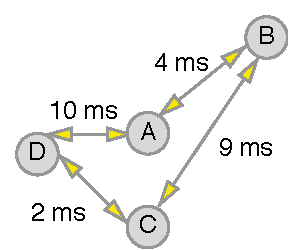
\includegraphics[width=3.4cm]{./FIGS/vivaldi_before.pdf}

%    \hspace*{0.5cm}
% 		\caption{Vivaldi plot before updating positions. Each node pings other nodes. Each node maintains a map of distance.}
% \label{fig:vivaldi_before}
%    \end{minipage}
% \hspace*{0.6cm}
%    \begin{minipage}[c]{.45\linewidth}
%    	\centering 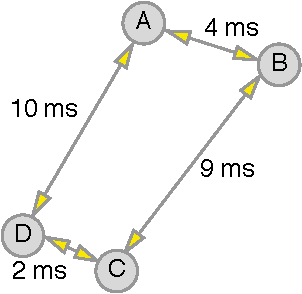
\includegraphics[width=3.4cm]{./FIGS/vivaldi_after.pdf}
% 		\caption{Vivaldi plot after updating positions. The computed
%                   positions of other nodes have been updated.}
% 		\label{fig:vivaldi_after} 
%   \end{minipage} \hfill
% \end{figure}

\subsubsection*{Searching for Close Nodes.}

Once the Vivaldi map is achieved, and each node knows its coordinates, we are
able to estimate how \emph{close} two given nodes are by calculating their
distance in the map. However, recall that the view of each node does not \emph{a
priori} contain its closest nodes \footnote{In the following, we call this view the {\bf
network view}, to distinguish it from the {\bf spiral view} to be introduced
later.}. Therefore, we need additional mechanisms to locate a set of nodes that
are close to a given initial node. Vivaldi gives a \emph{location} to each node,
not a neighborhood. 

We use a modified, distributed version of the classic Dijkstra's shortest path
algorithm that leverages the Vivaldi map to build such a neighborhood. More
specifically, its goal is to build a {\bf spiral}\footnote{Our use of the term
\emph{spiral} is actually a misuse of language, since the graph drawn in the
plane might contain crossing edges.} interconnecting the nodes in the plane that
are the closest ones from a given initial node.

Let us consider that our initial (or root) point is the node $n_R$. The first
step is to find a node to build a two-node spiral starting with $n_R$. This is
done by selecting the node from $n_R$'s network view, say $n_i$, which exhibits
the smallest distance with $n_R$. $n_i$ becomes the second node in the
spiral. From this point on, $n_R$ remembers $n_i$ as its successor and $n_i$
remembers $n_R$ as its predecessor. $n_R$ also sends its network view to $n_i$,
which, on receipt, creates its {\bf spiral view} that contains the $N$ nodes
closest to $n_R$ taken from both $n_R$ and $n_i$ network views. It will allow
$n_i$ to find the next node to build the spiral. Assuming this closest node from
$n_R$ in $n_i$'s spiral view is $n_j$, $n_j$ will be added in the spiral by
becoming the successor of $n_i$. $n_j$ receives $n_i$'s spiral view and creates
and fills its own spiral view with nodes closest to $n_R$ contained in both
$n_i$'s spiral view and $n_j$'s network view. This algorithm is repeated until
the amount of nodes requested by the application have been interconnected in the
spiral.

Note that there is a risk to be blocked at some point, having a spiral view
containing only nodes that are already in the spiral, hindering from extending
it further. However, this problem can be easily addressed by introducing few
long-distance nodes when the spiral view is created/updated.

\begin{figure}[ht]
  {
    \begin{center}{
	\begin{minipage}{.3\linewidth}
	  \begin{center}
	    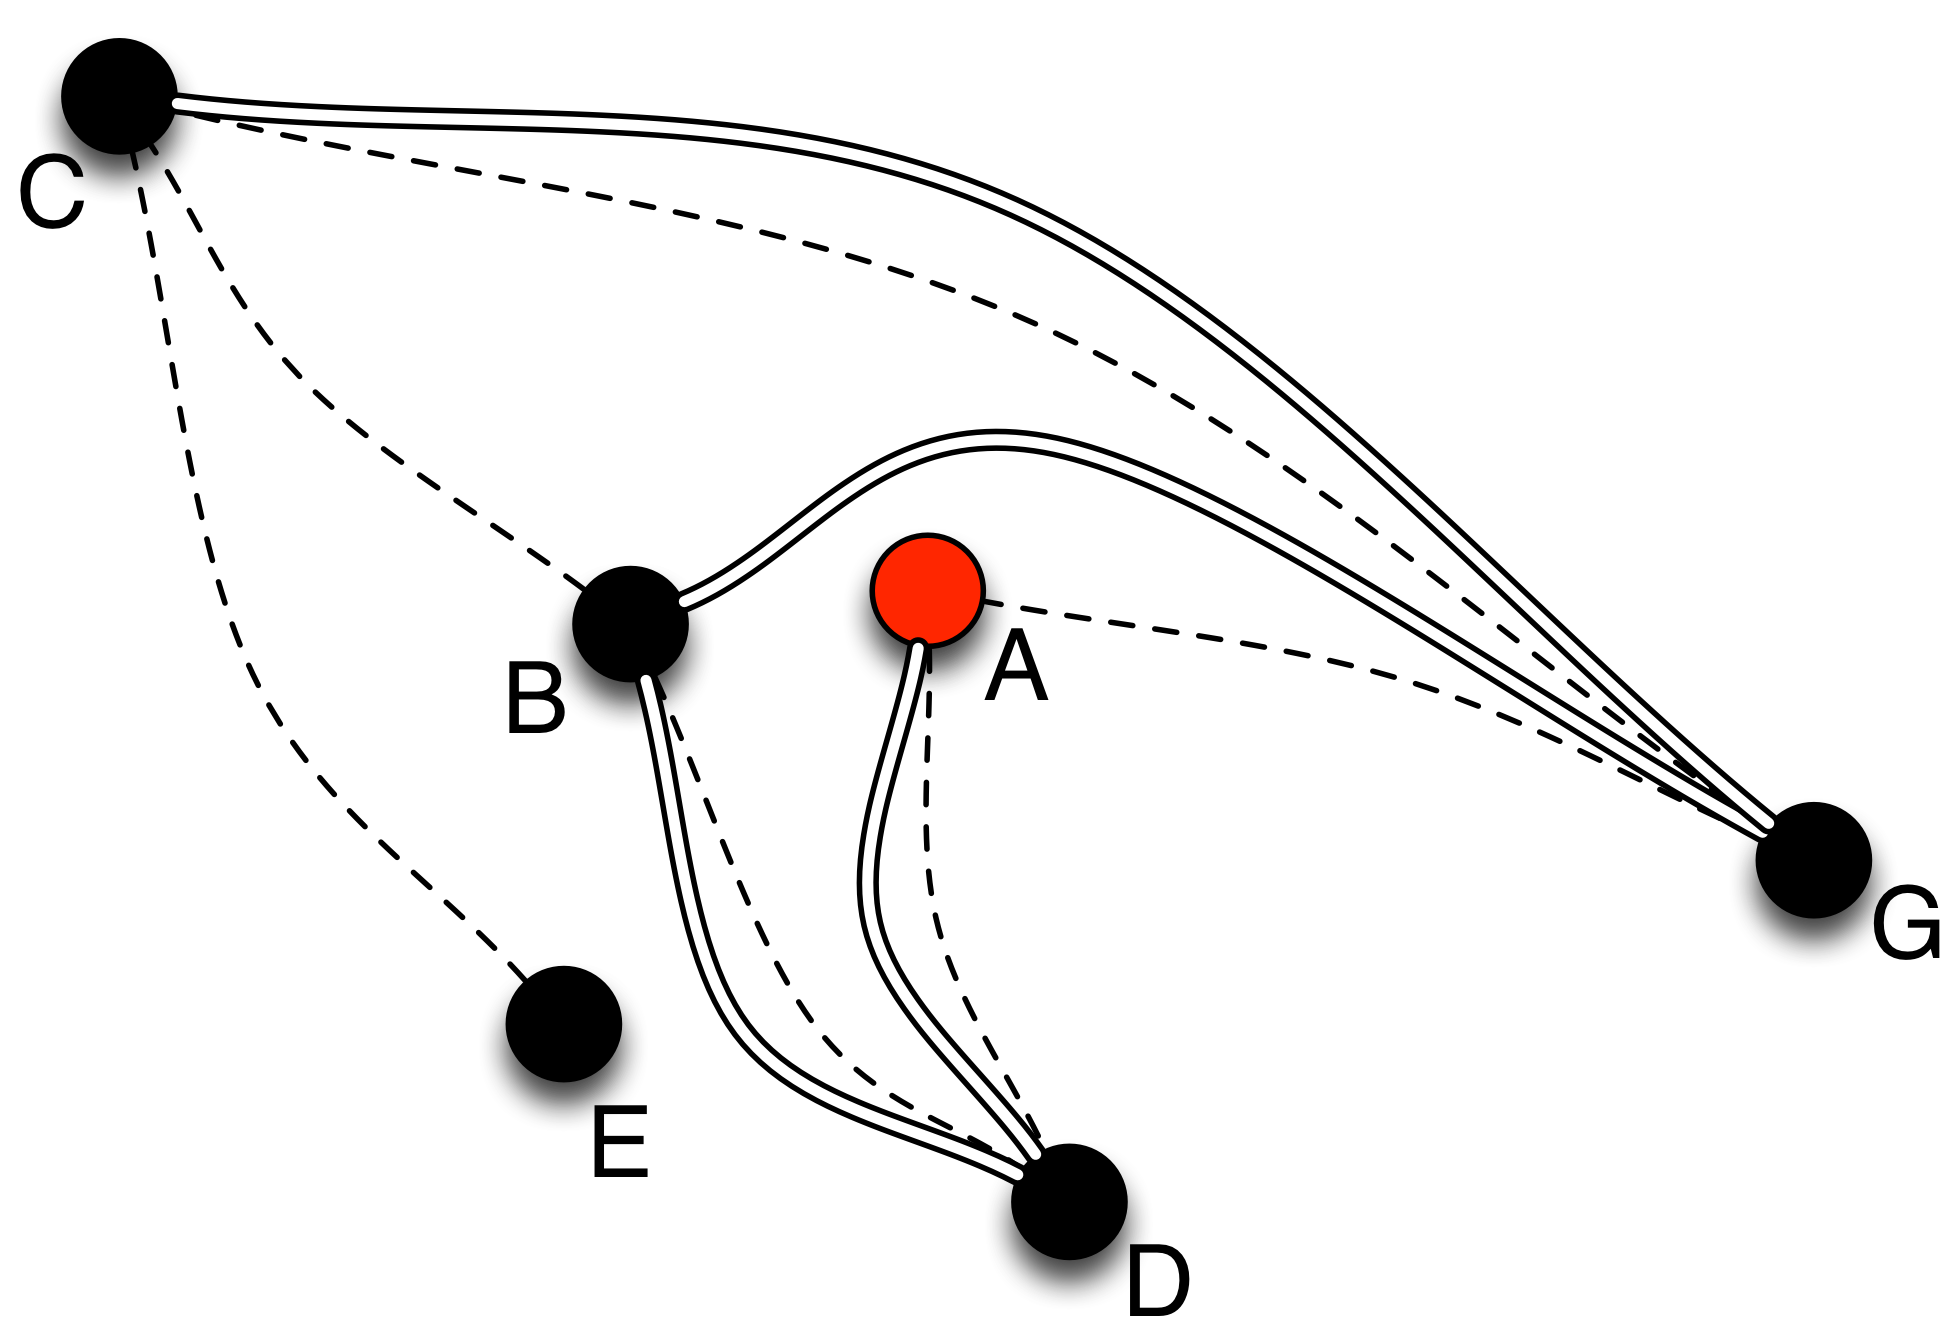
\includegraphics[width=1.05\linewidth]{Figures/learning1.png}\\(a)
	  \end{center}
	\end{minipage}
	~
	\begin{minipage}{.3\linewidth}
	  \begin{center}
	    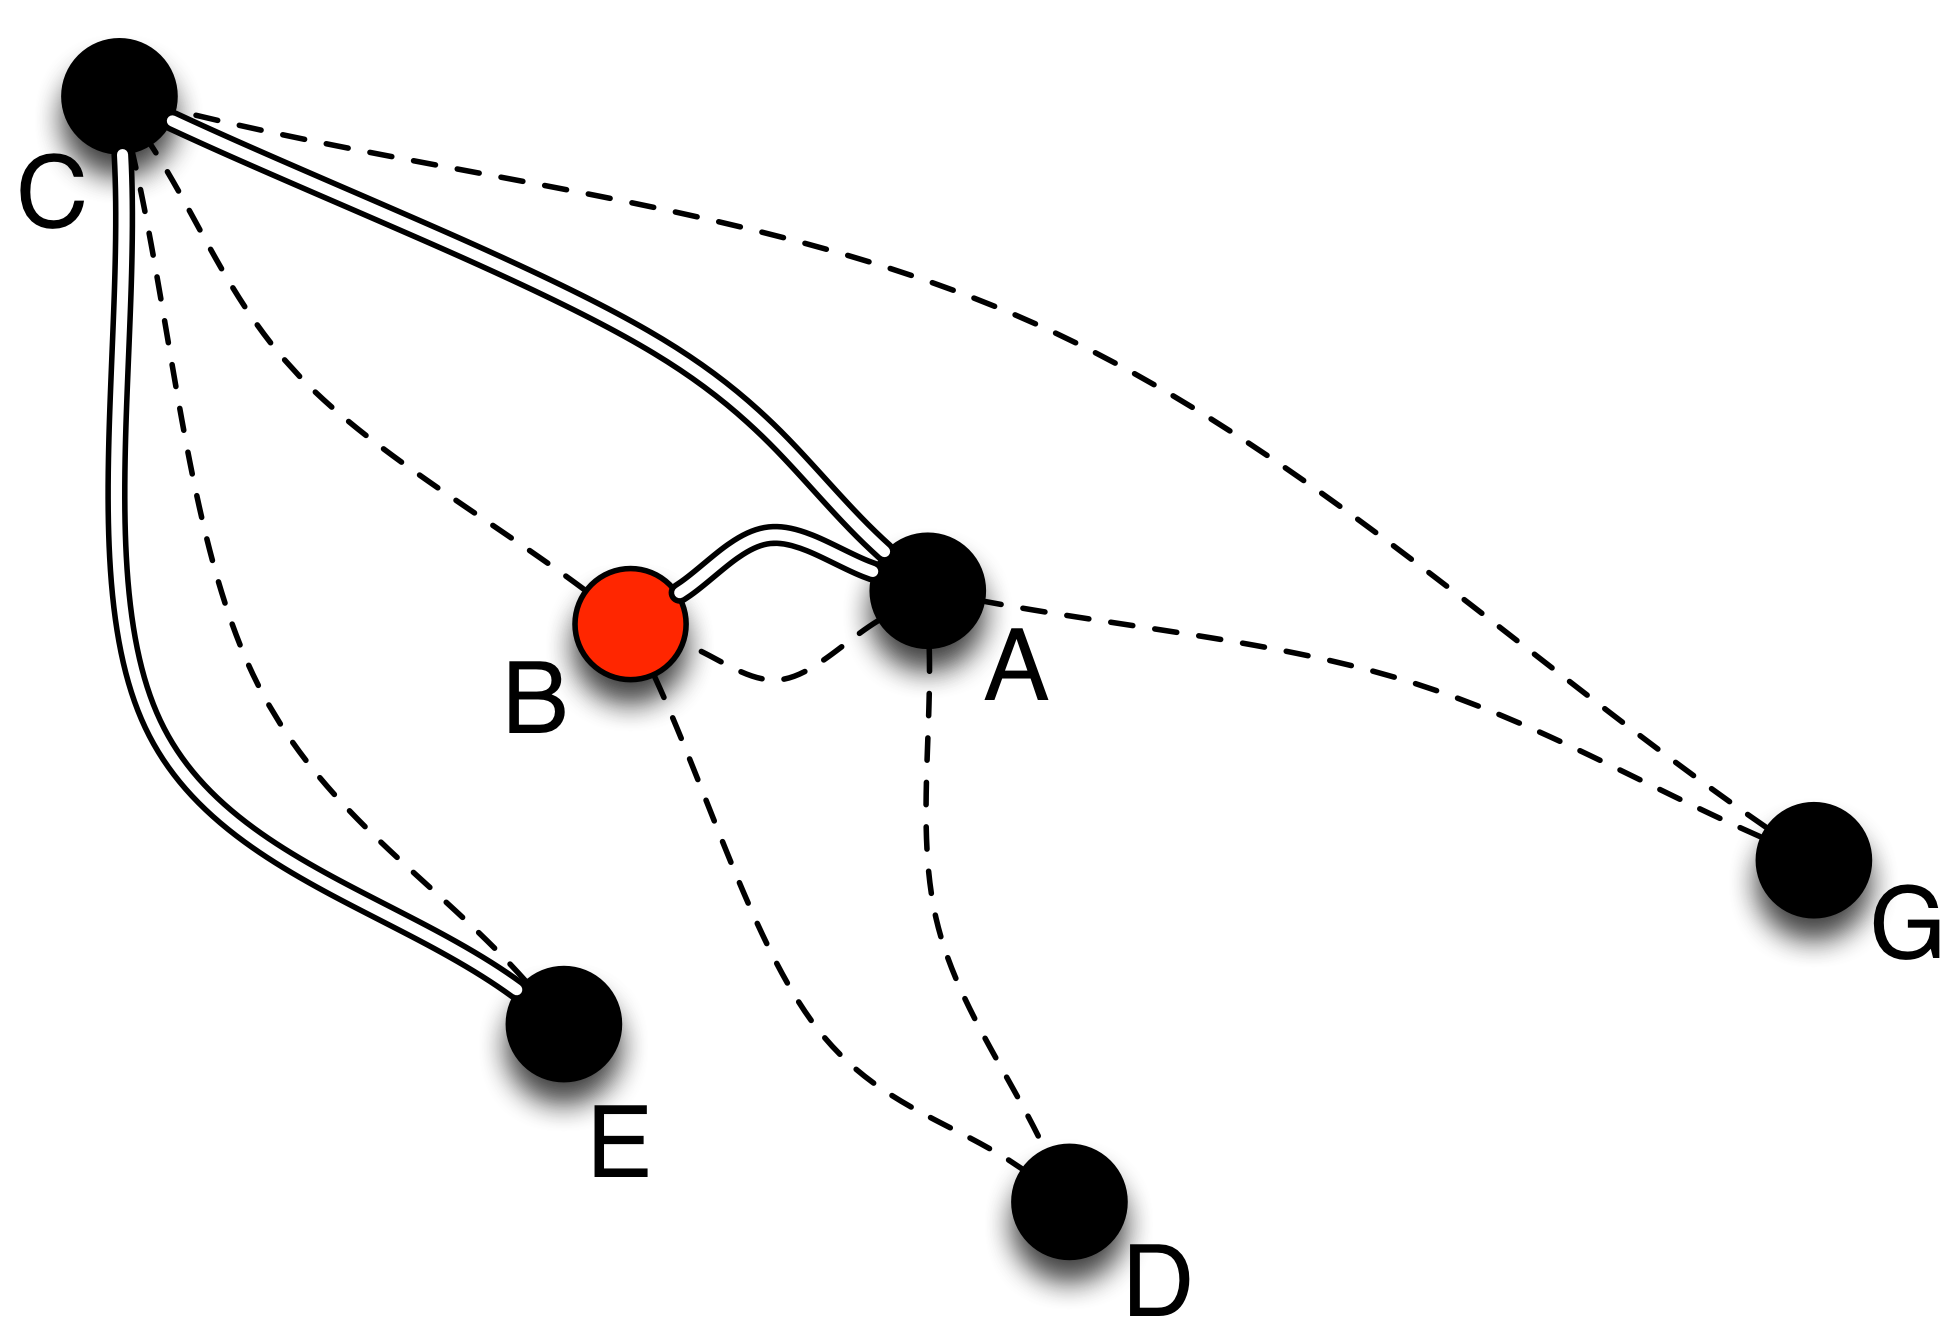
\includegraphics[width=1.05\linewidth]{Figures/learning2.png}\\(b)
	  \end{center}
	\end{minipage}
        ~
	\begin{minipage}{.3\linewidth}
	  \begin{center}
	    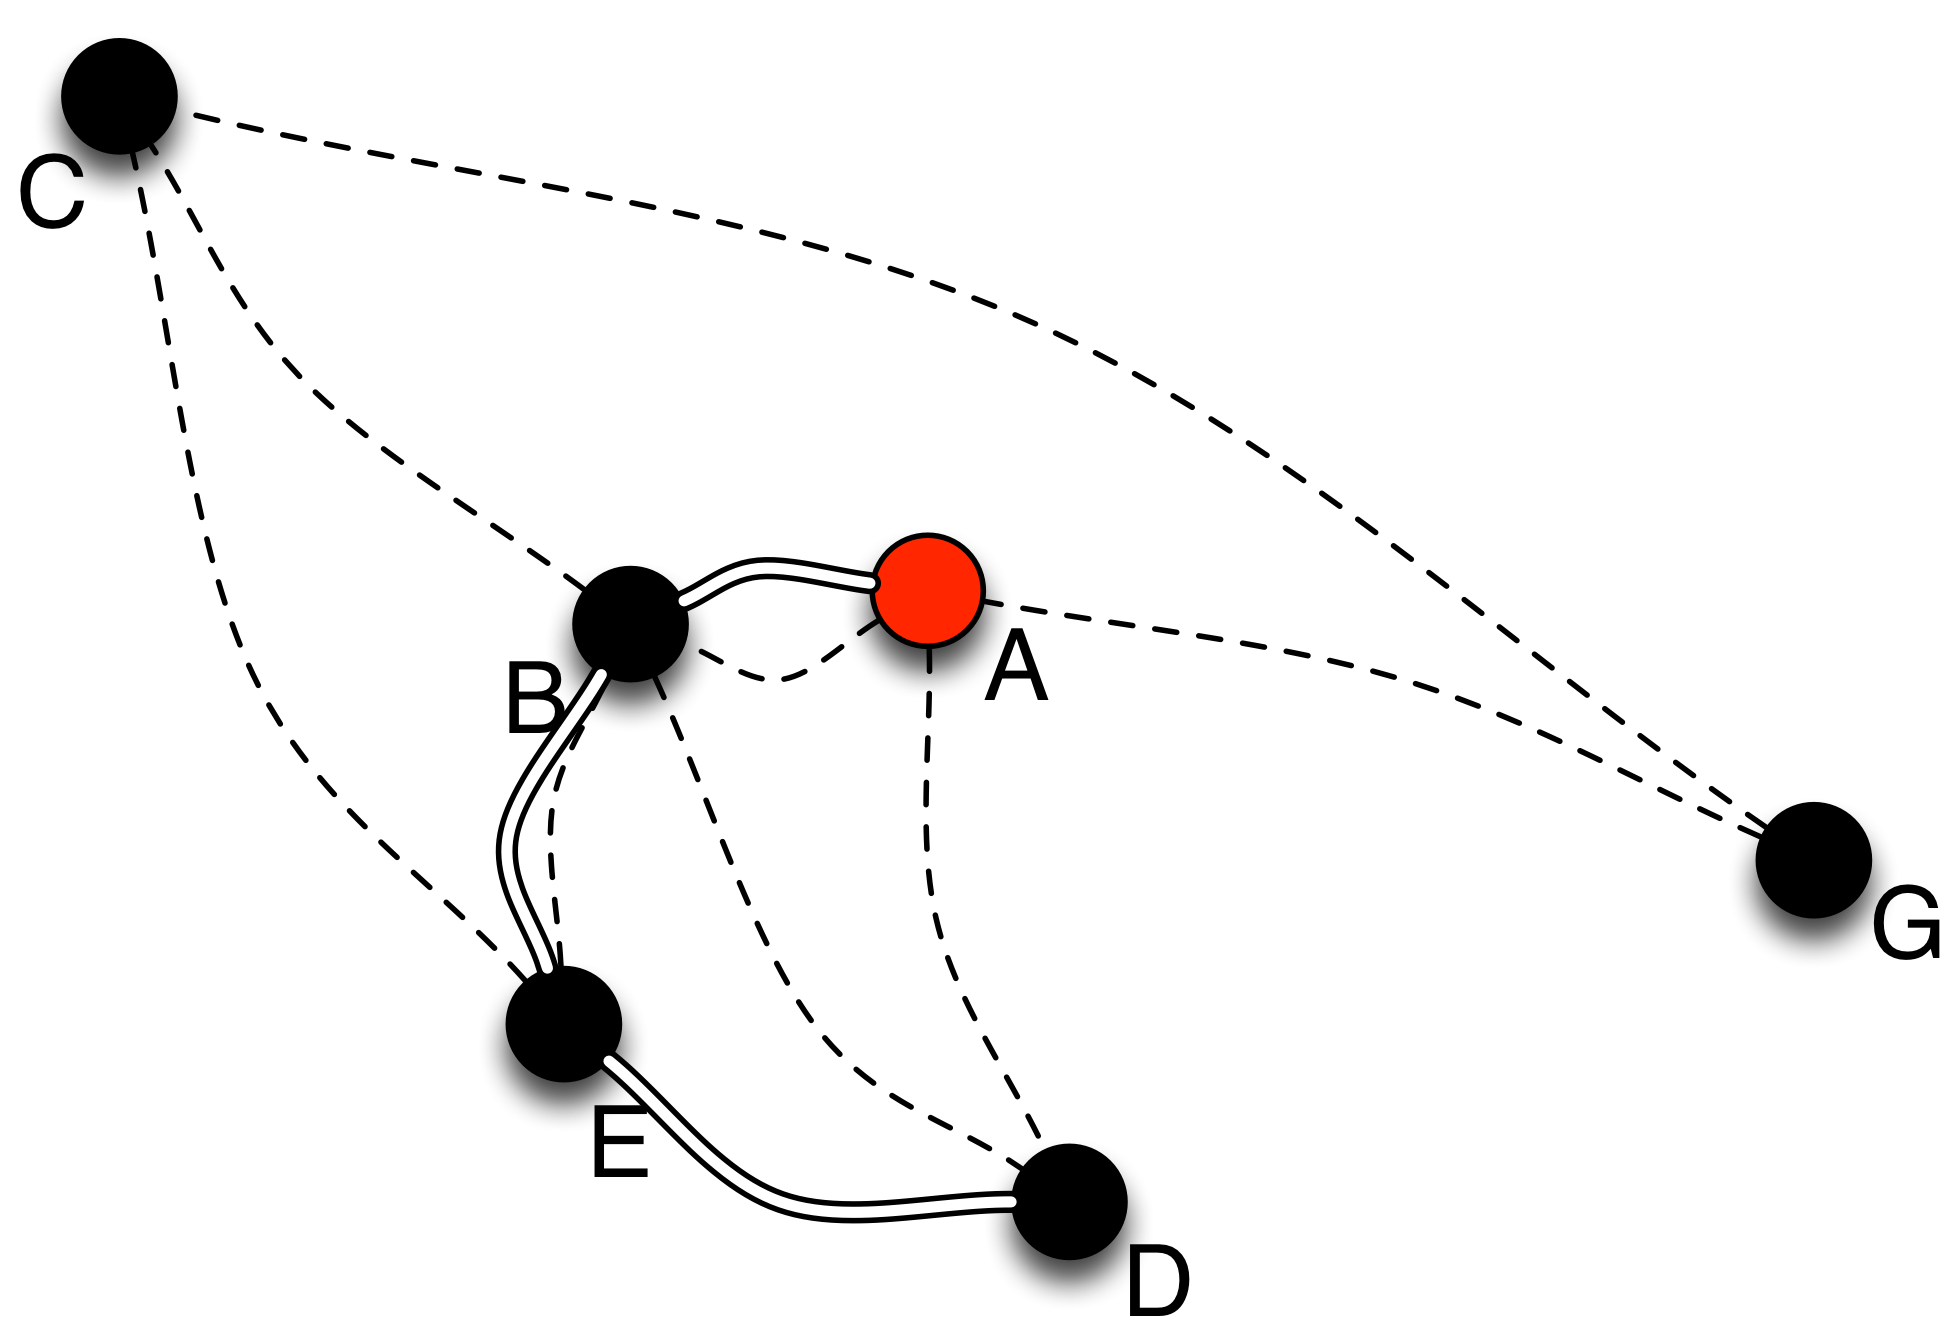
\includegraphics[width=1.05\linewidth]{Figures/learning3.png}\\(c)
	  \end{center}
	\end{minipage}
	\caption{Learning mechanism: (a)~The initial view of each node is materialized by
          the dashed lines. Given these views, the spiral obtained from node~A is
          represented by the double thick lines. In particular, this spiral allowed $A$
          and $B$ to discover each other. (b)~If $B$ starts building a spiral, it will
          start by contacting $A$. This spiral construction allows also E and B to
          discover each other. (c)~If $A$ is requested to start another spiral, it will
          exhibit an increased locality awareness.\label{fig:learning}} }
      \end{center}
}
\vspace*{-.8cm}
\end{figure}

\subsubsection*{Learning.}

Applying the protocol described above, the quality of the spiral is questionable in the
sense that the nodes that are actually close to the root node $n_R$ may not be
included.% The only property ensured is that one step
% forward on the built path always takes us further from the initial node.
%
To improve the \emph{quality} of the spiral, \ie to reduce the average
distance from each of its nodes to the initial node, we rely on a learning
mechanism coming with no extra communication cost: When a node is contacted to
become the next node in one spiral, and when it receives the associated spiral
view, it can also keep in its network view the nodes that are closer to itself,
thus potentially increasing the quality of a future spiral construction. Such an
improvement through learning is illustrated in Figure~\ref{fig:learning}. Note
that learning may also be used to constantly improve already built
spirals. While providing obvious advantages, allowing it comes at the cost of
changing links in the spirals dynamically, which may not match all applications'
constraints.

\subsection{PeerActor: A Building Block to Abstract Overlay Networks}
%
%%   * Construire des algos distribues fonctionnant en reseau est dur: couts 
%% 	  impliques par la tolerance aux pannes et synchro.
%%   * Ces couts sont parfois dus aux modeles de programmation.
%Building a distributed algorithm that works at large scale is complex: fault
%tolerance, synchronization and network overhead can have a cost that 
%significantly impact on performance and scalability. This can be the result of a
%bad software design, or the consequence of the use of an inapropriate 
%programming model for a given situation, as sharing states in a distributed
%context.
%
%%   * La collaboration entre processus peut se faire de deux maniere:
%%       A) partage d'etat.
%%       B) echange de message.
%This is especially true in situation where a process share a ressource with some 
%other processes. This situation, also known as \emph{race condition situation}, 
%has been thoroughly studied, which led to different ways to organize 
%collaboration between concurrent actors that have to work concurrently:
%
%\begin{description}
%
%	\item [Shared state] : A ressource is shared between different processes: it
%	requires that each process waits for its turn before acquiring it for use.
%	This property can be guaranteed by using locks to control acces to shared
%	ressource : processes have to wait that the ressource becomes free
%	before using it.
%
%	\item [Message passing] : Each process has its own state and collaborate
%	with other processes by exchange of messages. In the case of the actor model 
%	\cite{Hewitt1973}, a process becomes an \emph{actor} wich processes one
%	message at a time. This is a lock free approach with no	shared state.
%
%\end{description}
%
%%   * les verrous sont des nids a deadlocks.
%% 	* DVMS utilise le modele d'acteurs:
%%		- chaque instance ne communique qu'avec des messages.
%%		- on favorise les collaborations proches.
%Locking ressources often leads to deadlock \cite{agha:1986}, which can have
%a significant impact on performance and scalability. That is why we decided to
%leverage the actor model to reoarganize DVMS: each instance will collaborate
%by exclusively exchanging messages and priority will be given to collabarotion
%between close instances.
%
%%   * ainsi on a créé une librarie qui:
%%		- favorise le dvlpt d'appli distribuée.
%%		- se base sur des langages/frameworks modernes.
%%	* la librairie se base sur la prog fonctionnelle et le peerActor.
%With that in mind, we created a new library whose role is to ease the

%\begin{figure}[h!]
\begin{wrapfigure}[18]{r}{0.3\linewidth}
\vspace{-.7cm}\hspace*{.2cm}
  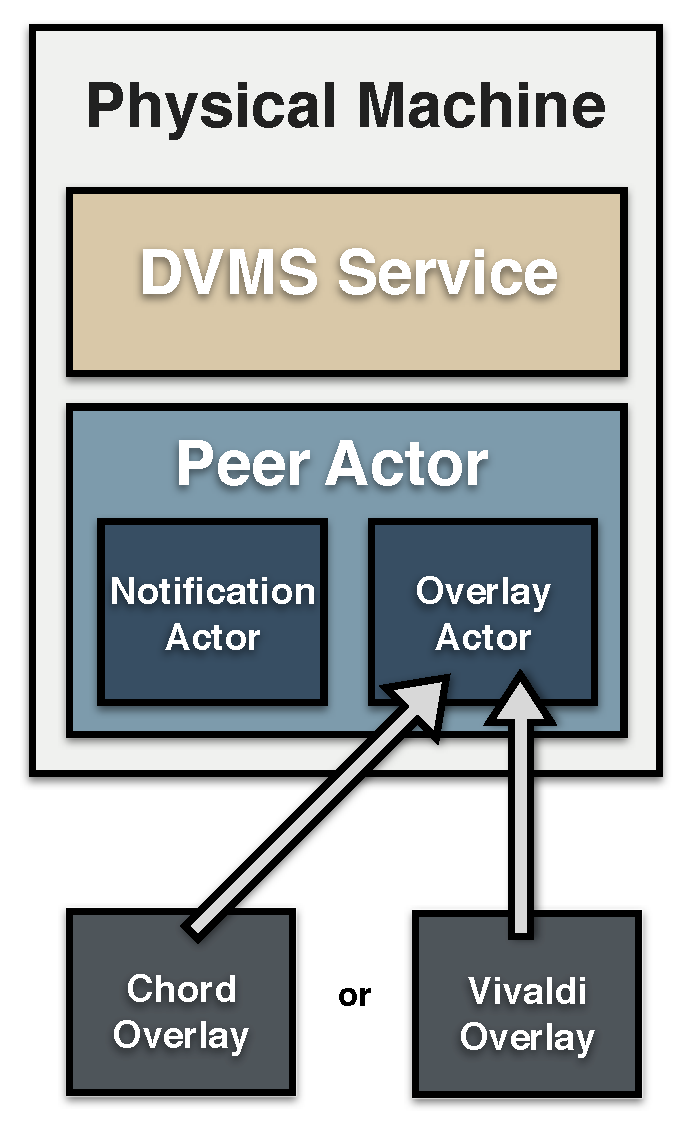
\includegraphics[width=\linewidth]{Figures/DVMS.pdf}
  \caption{DVMS on top of the Peer actor.}%
  \label{fig:peeractor}%
%\end{figure}
\end{wrapfigure}

As a P2P scheduling algorithm, the DVMS proposal can be divided in two major
components: (i)~The ring overlay network and (ii)~the protocol in charge
of detecting and resolving scheduling issues. As our goal consists in taking into account
locality criteria without changing the DVMS protocol, we designed a building block, \ie
\emph{the Peer actor}, which enables us to revisit DVMS by abstracting the overlay network it
relies on. At a coarse-grain level, the Peer actor can be seen as a generic layer for high
level distributed services, providing network abstractions and robust communications
between agents deployed on each node. By leveraging the Peer actor API, developers can
focus on the service itself without dealing with node apparitions/removals and network
disconnections.

From the software point of view, the Peer actor relies on modern software frameworks (Scala
and Akka) following the actor model rules. In such a model, each instance will
collaborate by exclusively exchanging messages, and priority will be given to collaboration
between close instances when using the locality-based overlay~(LBO).

%%\subsubsection{Peer actor abstraction}
%
%%   * Peer actor:
%%		- apporte la tolerance aux pannes, abstraction du réseau, communication
%%		  interservices.
%%		- propose une API pour développer vite.
%At coarse-grained, the \emph{Peer actor} provides several features: fault tolerance,
%network abstraction and communication between services.
%%   * Peer actor deux sous acteurs:
%%		- notification actor: systeme a evenement pour les services.
%%		- network overlay actor: réseau avec implémentation chord et vivaldi.

As illustrated in Figure~\ref{fig:peeractor}, the Peer actor contains two sub actors: The
\emph{Notification actor} and the \emph{Overlay network actor}. The Notification actor
enables services to subscribe to events that will be triggered by other services, as for detecting
overloading of nodes or for handling crash of neighbours. The
Overlay network actor is in charge of sending/receiving messages through the network. In order
to compare both approaches, ring-based \vs locality-aware, we developed two different
Overlay network actors: The first one provides a Chord-like overlay
\cite{stoica2001chord}, while the second one delivers the locality-aware overlay described
in Section~\ref{ssec:lao}.

